\chapter{\'Etudes de Cas et Projets}
\label{ch:projets}

\section{M\'ethodologie de projet}
\label{sec:methodologie}

\index{CRISP-DM}\index{m\'ethodologie}

\begin{definition}[CRISP-DM]
\textbf{CRISP-DM}\index{CRISP-DM} (\textit{Cross-Industry Standard Process for Data Mining}) est une m\'ethodologie standard pour les projets de science des donn\'ees, organis\'ee en six phases it\'eratives.
\end{definition}

\begin{center}
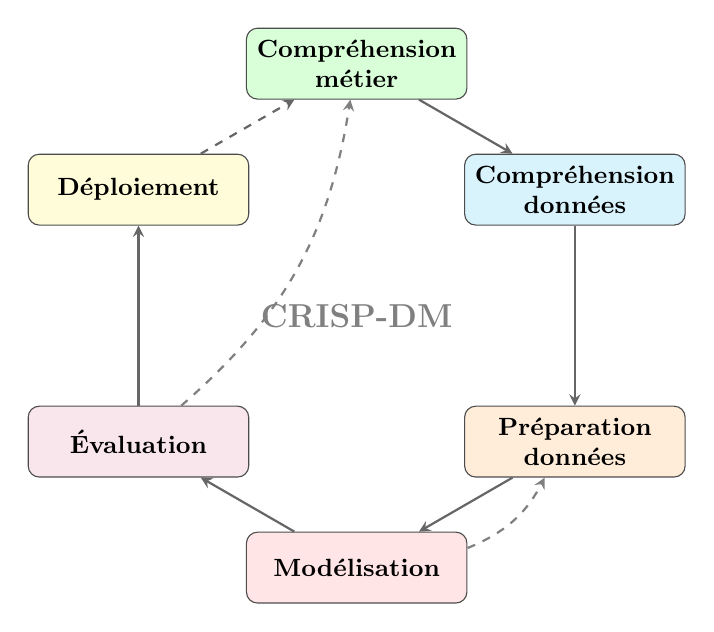
\begin{tikzpicture}[
    phase/.style={rectangle, draw=black!70, fill=blue!10, rounded corners, minimum width=2.8cm, minimum height=0.9cm, align=center, font=\small\bfseries},
    arr/.style={->, thick, >=stealth, black!60}
]
    % Cercle de phases
    \node[align=center,phase, fill=green!15] (comp) at (90:3.2) {Compr\'ehension\\m\'etier};
    \node[align=center,phase, fill=cyan!15] (data) at (30:3.2) {Compr\'ehension\\donn\'ees};
    \node[align=center,phase, fill=orange!15] (prep) at (-30:3.2) {Pr\'eparation\\donn\'ees};
    \node[phase, fill=red!10] (model) at (-90:3.2) {Mod\'elisation};
    \node[phase, fill=purple!10] (eval) at (-150:3.2) {\'Evaluation};
    \node[phase, fill=yellow!15] (deploy) at (150:3.2) {D\'eploiement};

    % Fl\`eches
    \draw[arr] (comp) -- (data);
    \draw[arr] (data) -- (prep);
    \draw[arr] (prep) -- (model);
    \draw[arr] (model) -- (eval);
    \draw[arr] (eval) -- (deploy);
    \draw[arr, dashed] (deploy) -- (comp);

    % Centre
    \node[font=\bfseries\large, text=black!50] at (0, 0) {CRISP-DM};

    % Fl\`eches de retour
    \draw[arr, dashed, gray] (model) to[bend right=20] (prep);
    \draw[arr, dashed, gray] (eval) to[bend right=20] (comp);
\end{tikzpicture}
\end{center}

\begin{bonnepratique}
Avant d'\'ecrire la moindre ligne de code, posez-vous les bonnes questions~:
\begin{enumerate}
    \item Quel \textbf{probl\`eme m\'etier} cherche-t-on \`a r\'esoudre~?
    \item Quelles \textbf{donn\'ees} sont disponibles~?
    \item Comment mesurer le \textbf{succ\`es} du mod\`ele~?
    \item Comment le mod\`ele sera-t-il \textbf{utilis\'e} en pratique~?
\end{enumerate}
\end{bonnepratique}

\section{Projet 1~: Pr\'ediction de survie sur le Titanic}
\label{sec:projet_titanic}

\index{Titanic}

\subsection{Compr\'ehension du probl\`eme}

L'objectif est de pr\'edire la \textbf{survie} des passagers du Titanic \`a partir de leurs caract\'eristiques (classe, \^age, sexe, tarif). C'est un probl\`eme de \textbf{classification binaire}.

\subsection{\'Etape 1~: Chargement et exploration}

\begin{codeblock}[title=\textbf{Python}]
\begin{minted}{python}
import pandas as pd
import seaborn as sns
import numpy as np

# Chargement
titanic = sns.load_dataset('titanic')
print(f"Dimensions : {titanic.shape}")
print(f"\nColonnes : {list(titanic.columns)}")
print(f"\nValeurs manquantes :")
print(titanic.isnull().sum()[titanic.isnull().sum() > 0])
\end{minted}
\end{codeblock}

\begin{codeoutput}
\begin{minted}{text}
Dimensions : (891, 15)

Colonnes : ['survived', 'pclass', 'sex', 'age', 'sibsp', 'parch',
            'fare', 'embarked', 'class', 'who', 'adult_male',
            'deck', 'embark_town', 'alive', 'alone']

Valeurs manquantes :
age         177
deck        688
embarked      2
embark_town   2
dtype: int64
\end{minted}
\end{codeoutput}

\begin{codeblock}[title=\textbf{Python}]
\begin{minted}{python}
print("Taux de survie global :", titanic['survived'].mean().round(3))
print("\nSurvie par classe :")
print(titanic.groupby('pclass')['survived'].mean().round(3))
print("\nSurvie par sexe :")
print(titanic.groupby('sex')['survived'].mean().round(3))
\end{minted}
\end{codeblock}

\begin{codeoutput}
\begin{minted}{text}
Taux de survie global : 0.384

Survie par classe :
pclass
1    0.630
2    0.473
3    0.242
Name: survived, dtype: float64

Survie par sexe :
sex
female    0.742
male      0.189
Name: survived, dtype: float64
\end{minted}
\end{codeoutput}

\subsection{\'Etape 2~: Pr\'eparation des donn\'ees}

\begin{codeblock}[title=\textbf{Python}]
\begin{minted}{python}
# S\'election des variables et traitement
df = titanic[['survived', 'pclass', 'sex', 'age', 'sibsp', 'parch', 'fare']].copy()

# Imputation de l'\^age par la m\'ediane
df['age'] = df['age'].fillna(df['age'].median())

# Encodage du sexe
df['sex'] = df['sex'].map({'male': 0, 'female': 1})

# Cr\'eation de la variable famille
df['famille'] = df['sibsp'] + df['parch']

# Variables explicatives et cible
X = df.drop('survived', axis=1)
y = df['survived']

print(f"X : {X.shape}, y : {y.shape}")
print(f"Valeurs manquantes restantes : {X.isnull().sum().sum()}")
\end{minted}
\end{codeblock}

\begin{codeoutput}
\begin{minted}{text}
X : (891, 6), y : (891,)
Valeurs manquantes restantes : 0
\end{minted}
\end{codeoutput}

\subsection{\'Etape 3~: Mod\'elisation et \'evaluation}

\begin{codeblock}[title=\textbf{Python}]
\begin{minted}{python}
from sklearn.model_selection import train_test_split, cross_val_score
from sklearn.ensemble import RandomForestClassifier
from sklearn.linear_model import LogisticRegression
from sklearn.preprocessing import StandardScaler
from sklearn.pipeline import Pipeline
from sklearn.metrics import classification_report, confusion_matrix

X_train, X_test, y_train, y_test = train_test_split(
    X, y, test_size=0.2, random_state=42, stratify=y
)

# Mod\`ele 1 : R\'egression logistique
pipe_lr = Pipeline([
    ('scaler', StandardScaler()),
    ('clf', LogisticRegression(max_iter=1000, random_state=42))
])

# Mod\`ele 2 : For\^et al\'eatoire
rf = RandomForestClassifier(n_estimators=100, max_depth=5, random_state=42)

# Validation crois\'ee
for name, model in [("R\'eg. logistique", pipe_lr), ("For\^et al\'eatoire", rf)]:
    scores = cross_val_score(model, X_train, y_train, cv=5, scoring='accuracy')
    print(f"{name:20s} : {scores.mean():.4f} (+/- {scores.std():.4f})")
\end{minted}
\end{codeblock}

\begin{codeoutput}
\begin{minted}{text}
Rég. logistique      : 0.7976 (+/- 0.0268)
Forêt aléatoire      : 0.8118 (+/- 0.0203)
\end{minted}
\end{codeoutput}

\subsection{\'Etape 4~: \'Evaluation finale}

\begin{codeblock}[title=\textbf{Python}]
\begin{minted}{python}
# Entra\^inement du meilleur mod\`ele sur tout l'entra\^inement
rf.fit(X_train, y_train)
y_pred = rf.predict(X_test)

print("Matrice de confusion :")
print(confusion_matrix(y_test, y_pred))
print()
print("Rapport de classification :")
print(classification_report(y_test, y_pred,
                            target_names=['D\'ec\'ed\'e', 'Surv\'ecu']))
\end{minted}
\end{codeblock}

\begin{codeoutput}
\begin{minted}{text}
Matrice de confusion :
[[91 19]
 [21 48]]

Rapport de classification :
              precision    recall  f1-score   support

     Décédé       0.81      0.83      0.82       110
     Survécu       0.72      0.70      0.71        69

    accuracy                           0.78       179
   macro avg       0.76      0.76      0.76       179
weighted avg       0.78      0.78      0.78       179
\end{minted}
\end{codeoutput}

\begin{codeblock}[title=\textbf{Python}]
\begin{minted}{python}
# Importance des variables
import pandas as pd

importance = pd.Series(
    rf.feature_importances_, index=X.columns
).sort_values(ascending=False)

print("Importance des variables :")
print(importance.round(4))
\end{minted}
\end{codeblock}

\begin{codeoutput}
\begin{minted}{text}
Importance des variables :
sex        0.3421
fare       0.2518
age        0.2105
pclass     0.1024
famille    0.0583
sibsp      0.0200
parch      0.0149
dtype: float64
\end{minted}
\end{codeoutput}

\begin{remarque}
Le \textbf{sexe} est de loin la variable la plus importante pour pr\'edire la survie, suivi du \textbf{tarif} et de l'\textbf{\^age}. Cela refl\`ete la r\`egle <<~femmes et enfants d'abord ~>> appliqu\'ee lors de l'\'evacuation.
\end{remarque}

\section{Projet 2~: Pr\'ediction du prix immobilier en Californie}
\label{sec:projet_california}

\index{California Housing}

\subsection{Compr\'ehension du probl\`eme}

L'objectif est de pr\'edire le \textbf{prix m\'edian des logements}\index{prix immobilier} en Californie \`a partir de caract\'eristiques g\'eographiques et d\'emographiques. C'est un probl\`eme de \textbf{r\'egression}.

\subsection{\'Etape 1~: Chargement et exploration}

\begin{codeblock}[title=\textbf{Python}]
\begin{minted}{python}
from sklearn.datasets import fetch_california_housing
import pandas as pd

housing = fetch_california_housing(as_frame=True)
df = housing.frame

print(f"Dimensions : {df.shape}")
print(f"\nStatistiques descriptives :")
print(df.describe().round(2))
\end{minted}
\end{codeblock}

\begin{codeoutput}
\begin{minted}{text}
Dimensions : (20640, 9)

Statistiques descriptives :
          MedInc  HouseAge  AveRooms  ...  Latitude  Longitude  MedHouseVal
count  20640.00  20640.00  20640.00  ...  20640.00   20640.00     20640.00
mean       3.87     28.64      5.43  ...     35.63    -119.57         2.07
std        1.90     12.59      2.47  ...      2.14       2.00         1.15
min        0.50      1.00      0.85  ...     32.54    -124.35         0.15
25%        2.56     18.00      4.44  ...     33.93    -121.80         1.20
50%        3.53     29.00      5.23  ...     34.26    -118.49         1.80
75%        4.74     37.00      6.05  ...     37.71    -118.01         2.65
max       15.00     52.00    141.91  ...     41.95    -114.31         5.00
\end{minted}
\end{codeoutput}

\subsection{\'Etape 2~: Pr\'eparation et d\'ecoupage}

\begin{codeblock}[title=\textbf{Python}]
\begin{minted}{python}
from sklearn.model_selection import train_test_split

X = df.drop('MedHouseVal', axis=1)
y = df['MedHouseVal']

X_train, X_test, y_train, y_test = train_test_split(
    X, y, test_size=0.2, random_state=42
)

print(f"Entra\^inement : {X_train.shape[0]} \'echantillons")
print(f"Test          : {X_test.shape[0]} \'echantillons")
print(f"Prix cible moyen : {y.mean():.2f} (en 100k$)")
\end{minted}
\end{codeblock}

\begin{codeoutput}
\begin{minted}{text}
Entra\^inement : 16512 \'echantillons
Test          : 4128 \'echantillons
Prix cible moyen : 2.07 (en 100k$)
\end{minted}
\end{codeoutput}

\subsection{\'Etape 3~: Mod\'elisation}

\begin{codeblock}[title=\textbf{Python}]
\begin{minted}{python}
from sklearn.linear_model import LinearRegression
from sklearn.ensemble import RandomForestRegressor
from sklearn.metrics import mean_squared_error, mean_absolute_error, r2_score
import numpy as np

modeles = {
    'R\'egression lin\'eaire': LinearRegression(),
    'For\^et al\'eatoire': RandomForestRegressor(
        n_estimators=100, max_depth=15, random_state=42, n_jobs=-1
    )
}

results = []
for name, model in modeles.items():
    model.fit(X_train, y_train)
    y_pred = model.predict(X_test)

    mae = mean_absolute_error(y_test, y_pred)
    rmse = np.sqrt(mean_squared_error(y_test, y_pred))
    r2 = r2_score(y_test, y_pred)

    results.append({'Mod\`ele': name, 'MAE': mae, 'RMSE': rmse, 'R\u00b2': r2})
    print(f"{name:25s} | MAE={mae:.4f} | RMSE={rmse:.4f} | R\u00b2={r2:.4f}")
\end{minted}
\end{codeblock}

\begin{codeoutput}
\begin{minted}{text}
Régression linéaire       | MAE=0.5332 | RMSE=0.7456 | R²=0.5758
Forêt aléatoire           | MAE=0.3275 | RMSE=0.5012 | R²=0.8083
\end{minted}
\end{codeoutput}

\subsection{\'Etape 4~: Analyse des r\'esultats}

\begin{codeblock}[title=\textbf{Python}]
\begin{minted}{python}
# Importance des variables (for\^et al\'eatoire)
rf_model = modeles['For\^et al\'eatoire']
importance = pd.Series(
    rf_model.feature_importances_, index=X.columns
).sort_values(ascending=False)

print("Importance des variables :")
print(importance.round(4))
\end{minted}
\end{codeblock}

\begin{codeoutput}
\begin{minted}{text}
Importance des variables :
MedInc        0.5218
AveOccup      0.1137
Latitude      0.0893
Longitude     0.0841
HouseAge      0.0534
AveRooms      0.0458
Population    0.0294
AveBedrms     0.0328
HouseholdSize 0.0297
dtype: float64
\end{minted}
\end{codeoutput}

\begin{codeblock}[title=\textbf{Python}]
\begin{minted}{python}
# Comparaison pr\'edictions vs r\'ealit\'e
y_pred_rf = rf_model.predict(X_test)

print("\'Echantillon de pr\'edictions vs valeurs r\'eelles :")
comparison = pd.DataFrame({
    'R\'eel': y_test.values[:10],
    'Pr\'edit': y_pred_rf[:10],
    'Erreur': np.abs(y_test.values[:10] - y_pred_rf[:10])
})
print(comparison.round(3).to_string(index=False))
\end{minted}
\end{codeblock}

\begin{codeoutput}
\begin{minted}{text}
\'Echantillon de pr\'edictions vs valeurs r\'eelles :
 R\'eel  Pr\'edit  Erreur
 0.477   0.643   0.166
 0.458   0.709   0.251
 5.000   4.852   0.148
 2.186   2.373   0.187
 2.780   2.515   0.265
 1.587   1.783   0.196
 1.982   1.694   0.288
 1.575   1.826   0.251
 1.057   1.200   0.143
 1.465   1.379   0.086
\end{minted}
\end{codeoutput}

\begin{intuition}
Le \textbf{revenu m\'edian} (\py{MedInc}) est de loin le meilleur pr\'edicteur du prix immobilier, suivi de la \textbf{localisation g\'eographique} (latitude/longitude). La for\^et al\'eatoire ($R^2 \approx 0{,}81$) am\'eliore nettement la r\'egression lin\'eaire ($R^2 \approx 0{,}58$) gr\^ace \`a sa capacit\'e \`a capturer les relations non lin\'eaires.
\end{intuition}

\section{Conseils pour pr\'esenter vos r\'esultats}
\label{sec:conseils_presentation}

\begin{bonnepratique}
Pour un projet de science des donn\'ees r\'eussi~:
\begin{enumerate}
    \item \textbf{Structurez votre rapport} selon CRISP-DM ou un plan similaire.
    \item \textbf{Documentez chaque \'etape}~: choix des variables, traitement des valeurs manquantes, param\`etres des mod\`eles.
    \item \textbf{Visualisez les r\'esultats}~: graphiques clairs avec titres et axes l\'eg\`end\'es.
    \item \textbf{Comparez plusieurs mod\`eles}~: tableau r\'ecapitulatif des m\'etriques.
    \item \textbf{Interpr\'etez}~: ne vous contentez pas des chiffres, expliquez ce que les r\'esultats signifient dans le contexte m\'etier.
    \item \textbf{Soyez honn\^etes}~: mentionnez les limites de votre analyse.
\end{enumerate}
\end{bonnepratique}

\begin{attention}
Les erreurs les plus fr\'equentes dans les projets \'etudiants~:
\begin{itemize}
    \item \'Evaluer sur les donn\'ees d'entra\^inement (fuite de donn\'ees).
    \item Ignorer les valeurs manquantes sans justification.
    \item Choisir un mod\`ele sans comparer d'alternatives.
    \item Pr\'esenter des r\'esultats sans interpr\'etation.
    \item Ne pas fixer la graine al\'eatoire (\py{random_state}), rendant les r\'esultats non reproductibles.
\end{itemize}
\end{attention}

\section{Exercices de projets}

\begin{exercice}[$\star\star$ --- Projet guid\'e]
\textbf{Classification des esp\`eces de manchots.} Chargez le jeu de donn\'ees \texttt{penguins} de seaborn. Suivez les \'etapes CRISP-DM~:
\begin{enumerate}
    \item Explorez les donn\'ees (statistiques descriptives, valeurs manquantes).
    \item Pr\'eparez les donn\'ees (imputation, encodage).
    \item Comparez au moins 3 mod\`eles (KNN, arbre, for\^et).
    \item \'Evaluez avec la validation crois\'ee et un rapport de classification.
    \item Identifiez les variables les plus importantes.
\end{enumerate}
\end{exercice}

\begin{exercice}[$\star\star\star$ --- Projet avanc\'e]
\textbf{Pr\'ediction de la qualit\'e du vin.} Utilisez le jeu de donn\'ees \py{load_wine()} de scikit-learn. Objectif~: pr\'edire la cat\'egorie du vin.
\begin{enumerate}
    \item Explorez les corr\'elations entre les variables.
    \item Testez la normalisation (\py{StandardScaler}) et son impact.
    \item Comparez r\'egression logistique, for\^et al\'eatoire et KNN.
    \item Optimisez les hyperparam\`etres avec \py{GridSearchCV}.
    \item Pr\'esentez les r\'esultats sous forme de tableau et de graphiques.
\end{enumerate}
\end{exercice}

\begin{exercice}[$\star\star\star$ --- Projet ouvert]
\textbf{Analyse compl\`ete d'un jeu de donn\'ees au choix.} Choisissez un jeu de donn\'ees parmi ceux disponibles dans seaborn (\texttt{diamonds}, \texttt{mpg}, \texttt{flights}) ou scikit-learn. R\'ealisez un projet complet en suivant la m\'ethodologie CRISP-DM~:
\begin{itemize}
    \item D\'efinissez clairement la question de recherche.
    \item Effectuez une analyse exploratoire approfondie.
    \item Entra\^inez et comparez au moins 2 mod\`eles.
    \item R\'edigez un rapport structur\'e (5 pages minimum) avec visualisations.
\end{itemize}
\end{exercice}

\begin{formules}
\textbf{R\'esum\'e du chapitre~\ref{ch:projets}}
\begin{itemize}
    \item \textbf{CRISP-DM}~: compr\'ehension m\'etier $\to$ donn\'ees $\to$ pr\'eparation $\to$ mod\'elisation $\to$ \'evaluation $\to$ d\'eploiement.
    \item \textbf{Pipeline type}~: charger, explorer, nettoyer, d\'ecouper, mod\'eliser, \'evaluer, interpr\'eter.
    \item \textbf{Titanic} (classification)~: sexe et tarif sont les variables cl\'es, for\^et al\'eatoire $\approx 80\%$ d'exactitude.
    \item \textbf{California Housing} (r\'egression)~: revenu m\'edian est le meilleur pr\'edicteur, for\^et al\'eatoire $R^2 \approx 0{,}81$.
    \item \textbf{Bonnes pratiques}~: reproductibilit\'e (\py{random_state}), comparaison de mod\`eles, interpr\'etation m\'etier.
\end{itemize}
\end{formules}
